%%%%%%%%%%%%%%%%%%%%%%%%%%%%%%%%%%%%%%%%%%%%%%%%%%%%%%%%%%%%%%%%%%%%%%%%%%
% Revisão Bibliográfica
%%%%%%%%%%%%%%%%%%%%%%%%%%%%%%%%%%%%%%%%%%%%%%%%%%%%%%%%%%%%%%%%%%%%%%%%%%

\chapter{Revisão Bibliográfica} \label{revisao}


Para esta seção, será conduzida uma revisão da literatura com o objetivo de explorar trabalhos relacionados ao desenvolvimento de compiladores para tradução de BRDFs expressas em \LaTeX{} para a linguagem de \textit{shading}, empregando técnicas de \textit{parsing}. O processo de busca será conduzido em duas etapas distintas. Inicialmente, será realizado um levantamento dos trabalhos existentes nas bases de dados  com relevantes periódicos, anais de eventos, artigos e trabalhos. Por fim, será realizada uma busca por produtos ou ferramentas similares no mercado, utilizando \textit{strings} de busca específicas em repositórios digitais, especificamente GitHub e SourceForge. Esses processos de busca permitirão identificar referências relevantes e estabelecer um panorama do estado da arte no campo dos compiladores de BRDFs  para \textit{shaders}, contribuindo para a compreensão do contexto acadêmico e prático no qual este trabalho se insere.


\section{Mapeamento Sistemático}


Com o intuito de obter resultados relevantes para a pesquisa, foram elaboradas frases de busca com base nos termos-chave relacionados ao tema deste trabalho. Também foram criadas questões de pesquisa para guiar a seleção dos trabalhos.


\subsection{Seleção das Bases}
As bases escolhidas foram: ACM Digital Library \footnote{\url{https://dl.acm.org/}},  IEEE Xplorer Digital Library \footnote{\url{https://ieeexplore.ieee.org/}},  Biblioteca Digital Brasileira de Teses e Dissertações (BDTD) \footnote{\url{https://bdtd.ibict.br/}}, Portal de Periódicos da CAPES \footnote{\url{https://www-periodicos-capes-gov-br.ezl.periodicos.capes.gov.br/index.php?}},  Google Acadêmico \footnote{\url{https://scholar.google.com/}}. Essas foram escolhidas por serem acessíveis gratuitamente pela afiliação à Universidade Federal de Sergipe, já o Google Scholar foi escolhido por agregar pesquisas em outras bases que possam ter trabalhos relevantes.


%
%


%
% \url{https://www-periodicos-capes-gov-br.ezl.periodicos.capes.gov.br/}








\subsection{Questões de Pequisa}  \label{questoes-pesquisa}


Foram elaboradas questões de pesquisa específicas que servem como guia para identificar e selecionar trabalhos científicos capazes de fornecer estratégias para o desenvolvimento do nosso projeto. Essas questões orientam a busca por artigos que apresentem soluções para desafios como: transformar descrições matemáticas de BRDFs em sequências computáveis adequadas para execução por renderizadores; representar modelos de \textit{shading} em estruturas hierárquicas; e desenvolver estratégias de compilação de BRDFs para linguagens de \textit{shading}. A partir desse processo, foram identificados e selecionados os trabalhos que melhor atendem às questões propostas, garantindo maior relevância para este estudo.


\begin{enumerate}
  \item Quais são as abordagens mais comuns utilizadas na criação de compiladores para tradução de BRDFs expressas em alguma linguagem de texto, como \LaTeX{}, para \textit{shaders}?

  \item Quais as técnicas de \textit{parsing} têm sido aplicadas no desenvolvimento de compiladores para linguagens matemáticas?

  %% @@@ Novo deve ser referenciado
  \item O trabalho utiliza gramáticas ou árvores de sintaxe para gerar/representar BRDFs ?

  %% @@@ Novo deve ser referenciado
  \item De que maneira é possível transformar BRDFs em representações hierárquicas estruturadas?

  %% @@@ Novo deve ser referenciado
  \item Como operações matemáticas de BRDFs podem ser decompostas em cálculos modulares, permitindo sua implementação em sistemas computacionais?

 \item Quais são os principais desafios enfrentados ao traduzir funções matemáticas complexas, como as BRDFs, em \textit{shaders}?

 \item Quais são as ferramentas e recursos disponíveis para auxiliar no desenvolvimento de compiladores para BRDFs e \textit{shaders}, e como eles podem ser integrados ao processo de desenvolvimento?

\end{enumerate}




\subsection{Termos de Busca}
 As frases foram construídas considerando suas variações equivalentes através de operadores lógicos. Posteriormente, as frases de pesquisa foram adaptadas de acordo com as características individuais de cada base de dados utilizada. Os termos-chave escolhidos foram: (("shader" OR "shading") AND "BRDF" AND ("compiler"\ OR "parser"\ OR "grammar")). As adaptações para cada base e o número de trabalhos encontrados são listados na \autoref{tab-bases}.



\begin{table}[H]
\ABNTEXfontereduzida
\caption{\small Tabela de pesquisa.}
\label{tab-bases}
\begin{tabular}{p{2.6cm}|p{6.0cm}|p{2.25cm}|p{3.40cm}}
  %\hline
   \textbf{Bases} & \textbf{Termos de Pesquisa}  & \textbf{Resultados}\\
   \hline
    IEEE Xplore Digital Library
    &
    ("Full Text \& Metadata":brdf)
AND (("Full Text \& Metadata":shader) OR  ("Full Text \& Metadata":shading))
AND (("Full Text \& Metadata":compiler) OR  ("Full Text \& Metadata":parsing) OR  ("Full Text \& Metadata":parser) OR  ("Full Text \& Metadata":grammar))
   & 36
    \\ \hline


    BDTD
    & (Todos os campos:compiler OU Todos os campos:parsing OU Todos os campos:parser OU Todos os campos:compilador) E (Todos os campos:shader OU Todos os campos:shading) E (Todos os campos:brdf)
    & 0
    \\ \hline
    CAPES Periódico
    &  Qualquer campo contém brdf E 
 Qualquer campo contém compi* E shad*  
    & 0
    \\ \hline


  ACM Digital Library
  & AllField:((shader OR shading) AND brdf AND (compiler OR compiling) AND (parser OR grammar OR parsing))
  & 46
    \\ \hline


 Google Acadêmico
  & 
  ("BRDF" AND ("COMPILER" OR "COMPILING") AND( "PARSER" OR "PARSING") AND ("SHADER" OR "SHADING"))
  & 69
   % \hline
\end{tabular}
\end{table}


\subsection{Critérios}


Para garantir a relevância dos resultados obtidos, seguimos os critérios de inclusão e exclusão estabelecidos, de forma a filtrar os resultados. Ao fim desse procedimento, apenas os resultados com maior compatibilidade com este trabalho foram analisados e descritos de maneira detalhada. O resultados se encontram na \autoref{tab-result}.


\subsubsection{Critérios de Inclusão}


\begin{enumerate}
  \item Foram incluídos artigos relacionados às palavras-chaves;

  \item Foram incluídos artigos que de alguma forma citem a criação de um compilador ou um \textit{parser};

  \item Foram incluídos artigos que utilizam representações hierárquicas para BRDFs, pois contribuem para a compreensão de como decompor BRDFs em estruturas adequadas para o nosso compilador, que é baseado em árvores.

  \item Foram incluídos artigos que apresentam linearização de BRDFs em sequências computáveis, relevantes para a geração de código a partir de árvores sintáticas.
\end{enumerate}


\subsubsection{Critérios de Exclusão}


\begin{enumerate}
  \item Foram excluídos artigos que dispunham de \textit{links} incorretos e ou quebrados;
  \item Foram excluídos artigos que não estão relacionados com as questões de pesquisa da \autoref{questoes-pesquisa};
  % \item Foram excluídos artigos que não têm como entrada uma BRDF no formato de equação, ou seja, utilizam a representação diretamente como código;
  \item Foram excluídos artigos que não abordam nenhum dos seguintes aspectos: a geração de \textit{shaders} como saída, a estruturação hierárquica de BRDFs ou a decomposição das operações matemáticas associadas a BRDFs;

  \item Foram excluídos artigos que não citam BRDFs e compilador ou árvores em seu resumo;
  \item Se, após a leitura completa, o artigo não concerne os interesses deste trabalho, esse foi excluído.
\end{enumerate}




\begin{table}[H]
\ABNTEXfontereduzida
  \caption{\small Resultados das bases após aplicar os critérios.}
\label{tab-result}
\begin{tabular}{p{6.6cm}|p{6.6cm}}
  %\hline
   \textbf{Bases}  & \textbf{Filtrados}\\
   \hline
    IEEE Xplore Digital Library
    % NOTE: Eram 2, mas removi 'Tree-Structured Shading Decomposition'.
   & 1 
    \\ \hline
    BDTD
    & 0
    \\ \hline
    CAPES Periódico
    & 0
    \\ \hline


  ACM Digital Library
  & 1
    \\ \hline
 Google Acadêmico
  & 1
   % \hline
\end{tabular}
\end{table}





\subsection{Descrição dos Trabalhos Relacionados}


\subsubsection{genBRDF: Discovering New Analytic BRDFs with Genetic Programming}


Neste artigo é introduzido um \textit{framework} chamada genBRDF, a qual aplica técnicas de programação genética para explorar e descobrir novas BRDFs de maneira analítica \cite{genbrdf}. O processo inicia com a descrição analítica de uma BRDF existente\footnote{As BRDFs de entrada são escritas na linguagem definida pela gramática apresentada pelos autores, que permite operações matemáticas, como \verb"sin", \verb"cos", \verb"tan", \verb"exp", \verb"asin", \verb"acos", \verb"dot", \verb"+", \verb"sqrt". Como exemplo, os autores ilustram ${brdf}_{init} = \rho_s \cos(R \cdot V)^\alpha$, como uma BRDF válida.}, e interativamente aplica mutações e recombinações de partes das expressões matemáticas que compõem essas BRDFs à medida que novas gerações surgem.

Essas mutações são guiadas por uma função \textit{fitness}.
Esse tipo de função atua como o inverso de uma função de erro, sendo baseada em um \textit{dataset} de materiais previamente medidos. Ela direciona as mutações ao avaliar a qualidade das expressões geradas, permitindo que o \textit{framework} identifique as soluções viáveis após analisar milhares de variantes.

Os autores geraram uma gramática que inclui constantes e operadores matemáticos comuns encontrados em equações de BRDFs. A gramática é compilada, e a árvore sintática resultante passa por modificações realizadas pelo algoritmo genético. Nós na árvore podem ser trocados, substituídos, removidos e novos nós podem ser adicionados. Esse processo, após refinamento e análise, resulta em novas BRDFs. Alguns dos novos modelos de BRDF apresentados no documento incluem exemplares que superam os modelos existentes em termos de precisão e simplicidade.
 
Esse artigo se concentra em automaticamente encontrar novos modelos analíticos de BRDF, em vez de compilar diretamente equações BRDF em linguagens de \textit{shading}. Embora a representação das expressões das BRDFs possa potencialmente inspirar o nosso trabalho, o principal objetivo do artigo difere do nosso tema.


\subsubsection{Slang: language mechanisms for extensible real-time shading systems}


O artigo descreve a linguagem \texttt{Slang}, uma extensão da amplamente utilizada linguagem de \textit{shading} HLSL, projetada para aprimorar a modularidade e a extensibilidade \cite{slang}. A abordagem de \textit{design} da \texttt{Slang} é baseada em dois princípios fundamentais: garantir compatibilidade com o HLSL existente sempre que possível e introduzir recursos inspirados em linguagens de programação \textit{mainstream}, visando facilitar a familiaridade e a intuição dos desenvolvedores. O compilador desenvolvido neste estudo é capaz de gerar código de \textit{shading} em HLSL, que pode ser compilado por um compilador de HLSL existente.

%%
O autor enfatiza que cada extensão da \texttt{Slang} foi projetada para permitir uma transição gradual a partir do código HLSL já desenvolvido, garantindo a compatibilidade com a maioria das construções sintáticas e semânticas da linguagem HLSL. Isso elimina a necessidade de uma migração completa. Algumas dessas extensões incluem: funções genéricas, estruturas genéricas e tipos que implementam interfaces específicas, semelhantes às interfaces em \texttt{Java}.

Um exemplo do uso de interfaces e funções genéricas em \texttt{Slang} é apresentado no \autoref{cod-sland}. Ao declarar a conformidade com a interface \texttt{IFoo}, a definição da estrutura \texttt{MyType} deve incluir um método chamado \texttt{myMethod}, com a assinatura correspondente àquela definida na interface \texttt{IFoo}. Já na função \texttt{myGenericMethod}, o parâmetro \texttt{arg} é genérico, permitindo maior flexibilidade na implementação.

\begin{codigo}[H]
  \caption{\small Código de interface em \texttt{Slang}. }
  \label{cod-sland}
\begin{lstlisting}[language=C, frame=none, inputencoding=utf8]
interface IFoo {
    int myMethod(float arg);
}

struct MyType : IFoo {
    int myMethod(float arg) {
        return (int)arg + 1;
    }
}

int myGenericMethod<T>(T arg) where T : IFoo {
    return arg.myMethod(1.0);
}
\end{lstlisting}
\end{codigo}

Enquanto o artigo tenta melhorar a flexibilidade e a extensibilidade dos sistemas de \textit{shading} em tempo real, o nosso trabalho se concentra na compilação de equações BRDF em linguagens de \textit{shading}. Embora ambos os projetos envolvam o uso de \textit{shaders} e a geração de código de \textit{shading}, as abordagens e os focos são distintos

%%%%%%%%%%%%%%%%%%%%%%%%%%%%%%%%%%%%%%%%%%%%%%%
%%%%%%%%%%%%%%% REMOVED FOR NOW %%%%%%%%%%%%%%%
%%%%%%%%%%%%%%%%%%%%%%%%%%%%%%%%%%%%%%%%%%%%%%%
% \subsubsection{Tree-Structured Shading Decomposition}
%
%
% Esse trabalho propõe uma abordagem para inferir uma representação de BRDF estruturada em árvore a partir de uma única imagem para o sombreamento de objetos \cite{tree_decomposition}. Em vez de usar representações paramétricas, como é comum, é proposta uma abordagem que utiliza uma representação em árvore de \textit{shading}, combinando nós básicos e métodos para decompor o \textit{shading} da superfície do objeto, representado na \autoref{fig_decomp}.
%
%
% \begin{figure}[H]
%         \caption{\label{fig_decomp} \small Exemplo de decomposição de BRDFs em nós de uma árvore.}
%         \begin{center}
%             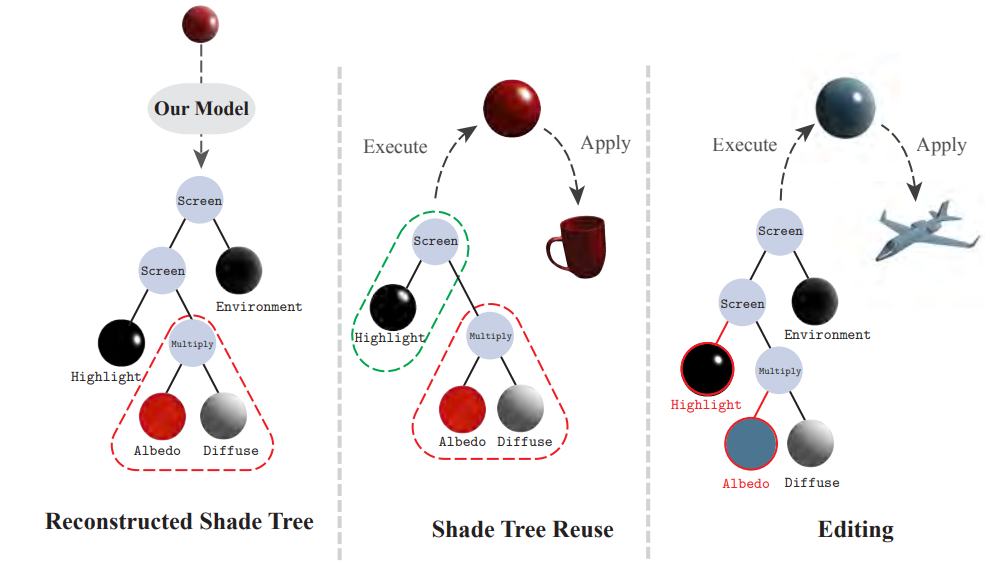
\includegraphics[scale=0.5]{./Imagens/tree-shading.png}
%         \end{center}
%         \legend{Fonte: \citeonline[]{radiometry_introduction}.}
% \end{figure}
%
%
%
%
% Assim como o nosso trabalho, esse artigo se concentra em facilitar o processo para usuários inexperientes, pois ambos visam fornecer ferramentas acessíveis para manipular representações de \textit{shading} sem exigir conhecimento avançado em programação. Esse artigo também emprega uma representação em árvore, embora para um propósito diferente.
%%%%%%%%%%%%%%%%%%%%%%%%%%%%%%%%%%%%%%%%%%%%%%%
%%%%%%%%%%%%%%% REMOVED FOR NOW %%%%%%%%%%%%%%%
%%%%%%%%%%%%%%%%%%%%%%%%%%%%%%%%%%%%%%%%%%%%%%%


\subsubsection{A Real-Time Configurable Shader Based on Lookup Tables}


Esse trabalho propõe uma arquitetura de \textit{hardware} que permite cálculos de \textit{shading} por pixel em tempo real, utilizando \textit{lookup-tables} \cite{configurable}. Para isso, são projetados circuitos configuráveis baseados nessas tabelas, memórias de acesso aleatório (RAMs) e memórias somente leitura (ROMs). Vários circuitos base foram projetados para as operações mais comuns, como o cálculo do produto interno entre dois vetores e a rotação de um vetor por um ângulo. Um exemplo desses diagramas é representado na \autoref{fig_circuit}. Ademais, foi utilizada interpolação em um sistema de coordenadas polares em vez da interpolação vetorial convencional, com o objetivo de reduzir o tamanho dos circuitos e melhorar o desempenho.

% Vários circuitos base foram projetados para as operações mais comuns, como o cálculo do produto interno entre dois vetores e a rotação de um vetor por um ângulo. Um exemplo desses diagramas é representado na \autoref{fig_circuit}. Além disso, foi utilizada interpolação em um sistema de coordenadas polares, em vez da interpolação vetorial convencional, com o objetivo de reduzir o tamanho dos circuitos e melhorar o desempenho




\begin{figure}[H]
        \caption{\label{fig_circuit}\small Exemplo de circuito de produto interno entre vetores.}
        \begin{center}
            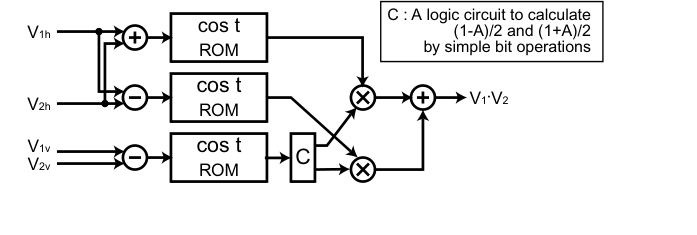
\includegraphics[scale=0.7]{./Imagens/rom-cos-lookup-table.png}
        \end{center}
  \legend{\small Fonte: \cite{configurable}.}
\end{figure}



Além disso, o circuito suporta diversas BRDFs, como Blinn-Phong, Cook-Torrance, Ward e modelos baseados em microfacetas, com tabelas específicas para cada modelo. O uso de tabelas de pesquisa permite a representação organizada da parametrização das BRDFs, tornando o processo de transformação de BRDF para \textit{shaders} mais acessível.

Este trabalho foi aceito por incluir o processo de tradução estruturada de BRDFs para uma sequência computável através de circuitos. Assim, o artigo demonstra como modularizar o cálculo das operações matemáticas contidas em BRDFs. A abordagem é útil para o nosso projeto, pois o processo de geração de \textit{shaders} a partir de uma árvore envolve linearizar as operações da BRDF em uma sequência correta, embora o propósito dessa tarefa em nosso projeto seja diferente do apresentado neste trabalho


\section{Pesquisa por Repositórios Online}
Também foram analisados repositórios no GitHub e SourceForge, cada um com uma \textit{string} de busca específica. Os repositórios encontrados foram filtrados baseados em seus resumos. Caso não haja a menção da criação de um compilador ou não seja citada uma transformação de BRDF para outra estrutura, esse repositório foi excluído. O resultado se encontra na \autoref{tab-repo}.




% @IMPORTANT 'preciso incluir o trabalho de conclusão de tulasi, que tem um repositório associado. Você pode colocar em uma seção diferente aqui neste capítulo. também é importante mencionar no capítulo 1 que esse trabalho existe, e que a abordagem do seu difere nas técnicas usadas.


\begin{table}[H]
\ABNTEXfontereduzida
\caption[bases]{\small Resultados da pesquisa nos repositórios.}
\label{tab-repo}
\begin{tabular}{p{2.6cm}|p{6.0cm}|p{2.25cm}|p{3.40cm}}
  %\hline
   \textbf{Plataformas} & \textbf{Termos de Pesquisa}  & \textbf{Resultados}\\
   \hline
   GitHub
   &
   in:readme (GLSL AND BRDF AND  (compiler OR compilation) AND (shader OR shading))
   & 15
   \\ \hline
   SourceForge
   &
   compiler bdrf
   & 0
\end{tabular}
\end{table}




Após ler por completo os resumos dos repositórios do GitHub, é evidente que nenhum desses projetos é relacionado com o proposto neste trabalho. Apesar de comentarem sobre BRDFs, esses projetos não implementam compiladores, não fazem \textit{parsing} de equações de BRDFs e nem mesmo geram \textit{shaders} a partir de BRDFs.

